\documentclass[12pt]{article}
% ====== Page Layout and Basic Formatting ======
\usepackage[left=1.0in,right=1.0in,top=1.0in,bottom=1.0in]{geometry}
\usepackage{setspace}
\doublespacing
\usepackage{fancyhdr}
\pagestyle{fancy}
\fancyhf{}
\fancyfoot[C]{\thepage}
\renewcommand{\headrulewidth}{0pt}

% ====== Typography and Fonts ======
\usepackage{lmodern}
\usepackage{microtype}
\usepackage[normalem]{ulem}
\usepackage[T1]{fontenc}

% ====== Section Styling ======
\usepackage{titlesec}
\usepackage[title]{appendix}
\usepackage{titling}
\pretitle{\begin{center}\large\bfseries}
\posttitle{\end{center}}
\preauthor{\begin{center}\normalsize}
\postauthor{\end{center}}
\predate{\begin{center}\normalsize}
\postdate{\end{center}}

% ====== Math Packages ======
\usepackage{amssymb, amsmath, amsfonts, mathtools}
% dsfont omitted — not in local TeX Live; we don't use blackboard digits in this paper
\usepackage{amsthm}
\newtheorem{theorem}{Theorem}
\newtheorem{proposition}{Proposition}
\newtheorem{corollary}{Corollary}
\newtheorem{lemma}{Lemma}
\newtheorem{definition}{Definition}

% ====== Table Packages ======
\usepackage{array, booktabs, makecell}
\usepackage{siunitx}
\usepackage[flushleft]{threeparttable}
\usepackage{tabularx}

% ====== Figure and Caption Packages ======
\usepackage{graphicx, subcaption}
% pdflscape, tikz omitted — no landscape or TikZ here
\usepackage{caption}
\captionsetup{font=small, labelfont=bf, justification=justified}
\usepackage{float}

% ====== List Formatting ======
\usepackage{enumitem}

% ====== Code listings ======
\usepackage{listings}
\usepackage{xcolor}
\definecolor{codebg}{rgb}{0.97,0.97,0.97}
\lstset{
  basicstyle=\ttfamily\small,
  backgroundcolor=\color{codebg},
  frame=single,
  framesep=4pt,
  breaklines=true,
  showstringspaces=false,
  columns=fullflexible,
}

% ====== Bibliography ======
\usepackage{xurl}
\definecolor{citationcolor}{RGB}{0, 127, 255}
\usepackage[backend=biber,
            style=authoryear,
            maxcitenames=3,
            mincitenames=1,
            maxbibnames=99,
            giveninits=true,
            uniquename=false,
            uniquelist=true,
            dashed=false,
            urldate=long,
            url=true,
            natbib=true]{biblatex}
\addbibresource{references.bib}
\renewcommand*{\nameyeardelim}{\addcomma\space}

% ====== Hyperref + cleveref ======
\usepackage[hidelinks, breaklinks, colorlinks=true,
            linkcolor=citationcolor, citecolor=citationcolor,
            urlcolor=citationcolor]{hyperref}
\usepackage[nameinlink]{cleveref}

% ====== Footnote settings ======
\interfootnotelinepenalty=10000
\setlength{\footnotesep}{0.5cm}

% ====== Title page metadata ======
\title{citecheck: A Free Tool for Detecting Retracted, Hallucinated, and Misattributed Citations in Academic Writing}

\author{
Pierre Beaucoral\thanks{Université Clermont Auvergne. Email: \href{mailto:pbeauco@gmail.com}{pbeauco@gmail.com}. Code and replication materials: \url{https://github.com/pierrebeaucoral/citecheck}.}
}

\date{\today}

\begin{document}

\maketitle
\thispagestyle{empty}

\begin{abstract}
\noindent \singlespacing
Large language models routinely fabricate bibliographic citations. \citet{walters_wilder_2023} document a fabrication rate of about 31\% in 636 ChatGPT-generated references; \citet{buchanan_hill_shapoval_2024} report a similar rate in economics. Existing tools that screen reference lists are either manual, paywalled, or limited to a single failure mode. This paper introduces citecheck, a free open-source tool that scans an academic PDF for two classes of problems: citations to retracted work and fabricated citations. The retraction check combines Crossref \texttt{update-to} with OpenAlex \texttt{is\_retracted}; the fabrication detector aggregates five signals (DOI integrity, cross-database existence, author plausibility, venue plausibility, and author--title coherence) into a rule-based verdict. On a labeled corpus of 770 references, citecheck attains precision of 0.551 and recall of 0.949 on the fabrication task. The pipeline runs locally on free public APIs.
\end{abstract}

\vspace{1em}
\noindent \textbf{JEL Codes:} C81, C88, O33

\vspace{0.5em}
\noindent \textbf{Keywords:} citation integrity, large language models, hallucination, retraction, open science

\newpage
\setcounter{page}{1}

% ============================================================
% SECTIONS — drafted by the writer agent. Markers below indicate
% the intended argument move for each section per writer.md.
% ============================================================

\section{Introduction}\label{sec:intro}

Large language models routinely produce text that includes bibliographic citations to works that do not exist. \citet{walters_wilder_2023} prompted ChatGPT-3.5 and ChatGPT-4 to generate scholarly essays on 42 topics and inspected the 636 resulting citations by hand. About 31\% referred to works that were entirely fabricated, and a further share contained substantive metadata errors. \citet{buchanan_hill_shapoval_2024} repeat the exercise in economics and report a fabrication rate close to 30\%. These rates are not artifacts of early model versions: similar findings have been replicated in medical, legal, and humanities settings since 2023. As LLM-assisted drafting moves from novelty to default, fabricated citations enter manuscripts, reviews, and downstream literature in volumes that manual screening cannot absorb.

Citations to retracted work pose a parallel problem. The Retraction Watch database, now distributed through Crossref since September 2023, catalogs more than 50{,}000 retracted articles. Recent estimates from the Retraction Watch team suggest that retracted papers continue to accrue citations long after the retraction notice is published, and that authors are typically unaware of the status of works they cite. Tools that screen for either problem exist (Scite.ai for citation context, Cabells for venue quality, Crossref's own retraction alerts), but most are commercial, restricted to institutional subscribers, or coupled to a single failure mode.

This paper describes citecheck, a free, open-source, locally runnable tool that scans an academic PDF for retracted and fabricated citations. The contribution is twofold. First, the tool combines five complementary detection signals on top of two free public APIs (Crossref and OpenAlex) and does not require an LLM at runtime. Four of the five layers are \emph{existence} checks (does this field appear in a database?) and one is a \emph{coherence} check (do two fields agree?), with a rule-based aggregator that weights coherence flags more heavily. Second, the aggregator implements an asymmetric low-coverage policy that suppresses false positives on legitimate older or un-indexed references, an empirical correction motivated by failures of the symmetric design on a known-good fixture. Evaluation uses a labeled corpus of 770 citations assembled from \citet{walters_wilder_2023} and two arXiv economics preprints whose reference lists serve as a real-by-construction control.

The rest of the paper is organized as follows. \Cref{sec:problem} states the three citation-integrity failure modes the tool targets and what is out of scope. \Cref{sec:tool} describes the pipeline. \Cref{sec:eval-set,sec:methodology} document the evaluation corpus and metrics. \Cref{sec:results} reports the headline numbers. \Cref{sec:discussion} discusses design choices and limitations. \Cref{sec:conclusion} concludes.

\section{The citation-integrity problem in the LLM era}\label{sec:problem}

A reference list can fail its readers in at least three ways. Citecheck targets two of them in the present release; the third is deferred to a later phase of development.

The first failure mode is citation to retracted work. A retraction notice is the scholarly record's way of marking a finding as withdrawn. Once a paper is retracted, a citation to it without acknowledgment of the retraction can mislead readers and propagate corrected or fraudulent results. The Retraction Watch database, the canonical registry of retraction events, became publicly accessible through Crossref in September 2023 \citep{retraction_watch}. Coverage is far from complete: Crossref's structured \texttt{update-to} field is populated only when the publisher deposits the retraction notice, which many publishers do not do for older works. The Wakefield 1998 MMR paper, retracted in 2010, is a canonical example: Crossref's \texttt{update-to} for the original article is empty, but OpenAlex's \texttt{is\_retracted} flag is true because OpenAlex merges Retraction Watch's manually curated list. No single source is sufficient.

The second failure mode is fabrication. A fabricated citation refers to a work that does not exist: the title, the authors, the year, or the venue are invented, or a real DOI is paired with an unrelated description. \citet{walters_wilder_2023} attribute roughly 31\% of 636 ChatGPT citations to outright fabrication; \citet{buchanan_hill_shapoval_2024} report comparable rates in economics. Fabrications are not random noise. They cluster on patterns that look plausible to a human reader: real-sounding journals, plausible authors, recent years. Detecting them by hand is costly; detecting them automatically requires a check that the cited entity actually appears in an external index.

The third failure mode is misrepresentation. A citation can refer to a real, un-retracted paper that does not in fact support the claim being made. This is the most consequential class of error in scientific writing, and the one that LLM drafting makes worst, because the language model is not constrained to read the cited paper before writing about it. Misrepresentation cannot be detected by metadata checks alone. It requires retrieving the cited paper's full text and comparing the claim to its content. Citecheck's Phase 5, scheduled after the present release, uses a local language model with retrieval-augmented generation to address misrepresentation. Phase 5 is out of scope for this paper; everything that follows concerns retraction and fabrication only.

\section{The citecheck pipeline}\label{sec:tool}

The tool runs as a command-line interface over a four-stage pipeline. Each stage produces a typed data object that the next stage consumes, so the pipeline can be inspected or replaced at any boundary. The stages are extraction, resolution, retraction check, and fabrication detection.

\paragraph{Stage 1: extraction.} A PDF is sent to a local instance of GROBID \citep{grobid}, an open-source conditional random field model for parsing scholarly documents. We use the \texttt{/api/processReferences} endpoint and request raw citation strings in the returned TEI XML. The non-obvious choice is \texttt{consolidateCitations=0}: GROBID supports calling Crossref during extraction to enrich metadata, and we explicitly disable it. Resolution is handled by the next stage with our own caching, scoring, and polite-pool headers; allowing GROBID to consolidate would bypass that control and double-count Crossref traffic. The parser keeps the subset of TEI fields needed to populate a typed \texttt{RawReference} record (title, authors, year, journal, DOI, raw citation string) and discards the rest.

\paragraph{Stage 2: resolution.} Each \texttt{RawReference} is mapped to a canonical DOI through a three-step dispatch. If the reference carries a DOI from GROBID's structured field or a regex over the raw text, citecheck queries Crossref's \texttt{/works/\{doi\}} endpoint directly. If no DOI is available, or the DOI lookup misses, citecheck queries Crossref's metadata search (\texttt{?query.bibliographic=...}) and scores candidates against the input. If Crossref returns no confident match, the dispatch falls back to OpenAlex \citep{openalex}. Both APIs are free; both honor a polite pool when the user sets \texttt{CITECHECK\_CONTACT\_EMAIL} in the environment, which citecheck attaches as a \texttt{mailto} parameter and in the user agent. The OpenAlex fallback is the engineering choice that matters: Crossref and OpenAlex are independently maintained indexes built from largely overlapping but non-identical sources, so a reference that misses both is far less likely to exist than one that misses only one.

\paragraph{Stage 3: retraction check.} For each resolved DOI, citecheck consults two sources and merges the results. The first is Crossref's \texttt{update-to} field, already cached on the reference from stage 2 at no extra request cost. Entries with types matching \texttt{retraction}, \texttt{withdrawal}, \texttt{expression-of-concern}, or \texttt{correction} are mapped to a structured status. The second is OpenAlex's \texttt{is\_retracted} boolean, which is populated from the Retraction Watch dataset distributed through the Crossref/Retraction Watch partnership since September 2023 \citep{retraction_watch,openalex}. Neither source alone is sufficient. Crossref's \texttt{update-to} is structured and dated when present, but is empty for many older retractions, including Wakefield's 1998 MMR paper. OpenAlex's flag is more complete but exposes neither the retraction notice DOI nor the date through the public works endpoint. The merge policy keeps both signals: the verdict takes the more severe status, and provenance fields fall back from Crossref to OpenAlex when Crossref is silent.

\paragraph{Stage 4: fabrication detection.} The fabrication detector aggregates five signals into a four-level verdict (\texttt{likely\_hallucinated}, \texttt{suspicious}, \texttt{real\_low\_confidence}, \texttt{real\_high\_confidence}). Each signal is cheap, returns a boolean flag, and is recorded in the output with a human-readable reason. The five signals fall into two categories. \emph{Existence checks} ask whether a field appears in a database; they are noisy because absence can mean obscurity rather than fabrication. \emph{Coherence checks} compare two fields against each other; they are stronger because absence of coherence between fields is hard to confuse with sparse coverage.

Layer L1 (DOI integrity) compares the metadata claimed by the citation to the metadata returned by Crossref for the same DOI. A title similarity below 75 (on the rapidfuzz token-set ratio) or a year discrepancy greater than one year flags the layer. A real DOI paired with a fabricated description is the classic signature of an LLM that pasted a plausible identifier under invented text.

Layer L2 (cross-database existence) reads the resolution status from stage 2. A reference that failed to resolve in both Crossref and OpenAlex is unlikely to be a real work; the layer flags \texttt{UNRESOLVED}. \texttt{AMBIGUOUS} status is informational and does not flag.

Layer L3 (author plausibility) queries OpenAlex's \texttt{/authors} endpoint for the first two listed authors. The layer flags only when both lookups miss. Single-author misses on non-English or junior researchers are common and not by themselves diagnostic.

Layer L4 (venue plausibility) queries OpenAlex's \texttt{/sources} endpoint for the claimed journal. A journal unknown to OpenAlex is a flag. The layer is skipped when the reference has no journal field, because books and working papers legitimately lack one.

Layer L5 (author--title coherence) is the second coherence check alongside L1. For each author who was located in L3, citecheck queries OpenAlex's \texttt{/works} endpoint filtered to that author's identifier and searched on the claimed title, then fuzzy-matches the top results. The layer flags when at least one author was found in L3 but none of those authors have an indexed work matching the claimed title. This catches the modal failure pattern documented by \citet{walters_wilder_2023}: real-author + invented-title combinations, where each field in isolation is plausible but the pairing is not. The layer is skipped when L3 found no authors (the redundant flag is suppressed) or when the citation has no claimed title.

The aggregator combines the five flags into a verdict. Four or more flags --- or three flags including at least one coherence flag (L1 or L5) --- produce \texttt{likely\_hallucinated}. Two flags or a single coherence flag alone produce \texttt{suspicious}. The remainder fall into \texttt{real\_high\_confidence} or \texttt{real\_low\_confidence} depending on whether resolution returned a DOI. The asymmetry between coherence and existence layers is what allows the detector to catch the modal LLM fabrication on articles: a real-author + invented-title combination that produces a single L5 flag with no other layer firing. A simple flag-counting rule that treated all five layers equivalently would miss those cases; an earlier version of the detector that did so missed almost every article-class fabrication in the eval set.

A low-coverage caveat applies to pre-2000 papers and references with no journal field. The caveat is asymmetric in a second sense. It downgrades \texttt{real\_high\_confidence} to \texttt{real\_low\_confidence} by one rank, but does not push \texttt{real\_low\_confidence} into \texttt{suspicious}; and it rolls back a \texttt{suspicious} verdict to \texttt{real\_low\_confidence} when the only flag is L5 on a reference with no journal (typically a book that OpenAlex does not index well). Both rules were empirically motivated. The original symmetric policy flagged the Hájek--Basu 1971 paper and the Neumark--Wascher MIT Press book in the Callaway--Sant'Anna \citep{callaway_santanna_2021_preprint} reference list as suspicious. Both are real. The asymmetric policy keeps the downgrade for high-confidence claims (we should be less sure about old or un-journaled work) without inflating the false-positive rate on the same class of references.

\paragraph{Design choices and what they cost.} Three choices in the pipeline are not the only reasonable ones and warrant brief justification.

First, the detector is rule-based rather than learned. A natural alternative is to train a binary classifier on labeled fabrications, or to ask a language model whether a citation looks real. Both are tempting. We rejected the trained-classifier path because labeled fabrication corpora are small and skewed --- \citet{walters_wilder_2023} is one of the few that exists in volume, and any classifier trained on it would memorize its idiosyncrasies. We rejected the language-model path because the cost structure (per-citation inference, in dollars or in tokens) defeats the project goal of a free, locally-runnable tool, and because a language model that fabricated citations to begin with is a brittle judge of which citations are fabricated. Rule-based aggregation is auditable: every flag has a reason, the thresholds are tunable, and the verdicts can be reproduced exactly from the same APIs. The cost is that the rules are heuristic; the eval set is what calibrates them.

Second, every detection step targets coverage in two databases (Crossref and OpenAlex). A single-source design would be simpler but brittle: Crossref's structured \texttt{update-to} for the Wakefield 1998 MMR paper is empty, OpenAlex's \texttt{is\_retracted} flag is true, and a single-source pipeline would miss one of those cases regardless of which source it picked. The two databases are independently maintained, drawn from largely overlapping but non-identical sources, and disagree in informative ways. We pay for this with extra requests per citation (the OpenAlex fallback for resolution, the OpenAlex queries for L3, L4, L5), all of which we cache aggressively with a seven-day TTL.

Third, fuzzy matching uses fixed thresholds (75 on the rapidfuzz token-set ratio for titles, 85 for author family names). These numbers were chosen empirically: a higher title threshold rejected too many real references whose GROBID-extracted title differed from the canonical Crossref title by a colon, a subtitle, or a typesetting artifact; a lower threshold accepted near-misses that should not have matched. The thresholds were not learned from the eval set --- they were set during the development of stage 2 on the Callaway--Sant'Anna fixture --- so the headline numbers do not reflect calibration on the data they are measured against. A more rigorous calibration on a held-out tuning split is on the roadmap, but the current values are defensible because no single decision in the detector hinges on a sharp boundary: a one-unit change in either threshold typically moves a handful of citations, not the headline verdict.

\section{Evaluation set}\label{sec:eval-set}

The evaluation corpus combines a primary public dataset with a domain-specific augmentation. Both sources are independent of citecheck's design, which matters: a hallucination detector evaluated on hallucinations generated by an LLM that thinks like the detector inherits the detector's blind spots.

The primary source is the supplementary appendix to \citet{walters_wilder_2023}. The authors prompted ChatGPT-3.5 and ChatGPT-4 to write scholarly essays on 42 topics, collected 84 essays containing 636 bibliographic citations, and inspected each citation against library catalogs and search engines. The supplementary spreadsheet records a per-citation \texttt{Work itself is fabricated} boolean, along with metadata, topic, model version, and the verification path used. Of the 636 citations, 441 refer to works that exist and 195 are fabricated. The file is distributed under CC-BY 4.0 and downloadable without authentication from the Springer static-content CDN. The 636 citations cover generalist humanities and scholarly topics; close to half of the cited works are books, which are indexed unevenly across Crossref and OpenAlex.

The augmentation set is 134 references extracted from the bibliographies of two arXiv economics preprints, \citet{callaway_santanna_2021_preprint} and \citet{borusyak_jaravel_spiess_2024_preprint}. These references are real by construction: they were submitted as citations in papers that have themselves been cited many times, so each reference has been read and checked by at least the author teams and by subsequent users of the methods. The augmentation set is labeled \texttt{real} for every row. Its purpose is twofold: it adds an economics-only slice to a Walters corpus that is humanities-leaning, and it provides a clean negative-class sample for measuring false-positive rate in a domain where citecheck is expected to be used.

Two independence properties are worth stating explicitly. First, the Walters citations were generated by ChatGPT and labeled by Walters and Wilder; citecheck had no role in either step. Citecheck is therefore being tested on a held-out distribution of natural LLM fabrications rather than on adversarial examples constructed against itself. Second, the augmentation references were not selected to exhibit any particular property: they are the full reference lists of two preprints widely used as methodological references in econometrics. Neither set was inspected during the design of the fabrication detector's thresholds.

The corpus has acknowledged limitations. It is humanities-heavy because Walters and Wilder's prompts target humanities and generalist topics. It is book-heavy because Walters and Wilder's prompts target a humanities readership and because LLMs in 2023 fabricated many of their citations as monographs. Crossref and OpenAlex both have weaker coverage of books than of journal articles, which means the fabrication detector's coverage proxies are noisier on this slice. The corpus is English-only and does not include medical or biological references. \Cref{tab:eval-sources} summarizes the composition.

\begin{table}[htbp]
\centering
\caption{Eval corpus composition}
\label{tab:eval-sources}
\begin{threeparttable}
\begin{tabular}{lcccc}
\toprule
Source                                   & Real & Fabricated & Total & Domain        \\
\midrule
\citet{walters_wilder_2023}              & 441  & 195        & 636   & Humanities/generalist \\
arXiv econ preprints (augmentation)      & 134  & 0          & 134   & Economics     \\
\midrule
Total                                    & 575  & 195        & 770   &               \\
\bottomrule
\end{tabular}
\begin{tablenotes}\small
\item \textit{Notes:} Walters counts taken from supplementary appendix 3 of \citet{walters_wilder_2023}, CC-BY 4.0. Augmentation set is the union of the reference lists of \citet{callaway_santanna_2021_preprint} and \citet{borusyak_jaravel_spiess_2024_preprint}, labeled \texttt{real} by construction.
\end{tablenotes}
\end{threeparttable}
\end{table}

Candidate sources for a v2 corpus, identified but not yet integrated, include \citet{buchanan_hill_shapoval_2024} for an economics slice, McGowan et al.\ (2023, \emph{Psychiatry Research}) for psychiatry, and JMIR Medical Informatics (2024) for open-access medical references. Each is documented in the eval-set source survey in the repository. The first is held up by the supplementary data being distributed as a single PDF; the others are scheduled for processing in the next release.

\section{Evaluation methodology}\label{sec:methodology}

The fabrication detector produces a four-level verdict, but evaluation reduces to a binary classification. The positive class is \emph{predicted fabricated}: verdicts \texttt{suspicious} or \texttt{likely\_hallucinated}. The negative class is \emph{predicted real}: verdicts \texttt{real\_high\_confidence} or \texttt{real\_low\_confidence}. The ground-truth label is the \texttt{Work itself is fabricated} flag from \citet{walters_wilder_2023} for the primary set and \texttt{real} by construction for the augmentation set. This collapse loses some information --- the four-level output communicates calibrated uncertainty to a human user --- but a binary framing is necessary to compute standard classification metrics against a binary label.

For each reference, citecheck outputs a verdict $\hat{y} \in \{0, 1\}$ where $\hat{y}=1$ denotes the positive class. The true label is $y \in \{0, 1\}$. The confusion matrix has four cells. True positives ($TP$) are fabricated references that citecheck flagged. False negatives ($FN$) are fabricated references citecheck called real. False positives ($FP$) are real references citecheck flagged. True negatives ($TN$) are real references citecheck called real. The reported metrics are precision $TP/(TP+FP)$, recall $TP/(TP+FN)$, false-positive rate $FP/(FP+TN)$, and the harmonic mean $F_1 = 2 \cdot \text{precision} \cdot \text{recall} / (\text{precision} + \text{recall})$.

Precision and false-positive rate carry different weights for the intended use. A user running citecheck on a draft manuscript will inspect the flagged references manually. A high false-positive rate forces the user to confirm legitimate citations and erodes trust in the tool. Recall matters most when the cost of missing a fabrication is high (a submission deadline, a peer-reviewed publication), but a missed fabrication is no worse than the status quo of unaided drafting. The asymmetric caveat in the aggregator (\cref{sec:tool}) explicitly trades a small amount of recall on books and pre-2000 papers for substantially lower false-positive rate on the same class. The empirical question is whether the trade is well calibrated; the metrics below adjudicate it.

Reproducibility is built into the repository. The script \texttt{scripts/build\_eval\_set.py} downloads the Walters and Wilder supplement, parses citation strings through GROBID's \texttt{processCitation} endpoint, and writes a \texttt{labels.csv} with stable row identifiers. The script \texttt{scripts/run\_eval.py} loads the labeled CSV, runs citecheck's fabrication pipeline against each row with a fixed seed for any randomized step, and writes a per-row prediction file alongside an aggregate metrics file. Cached API responses are stored in a SQLite database with a seven-day TTL, so reruns within that window do not re-query Crossref or OpenAlex. A complete replication consists of \texttt{uv sync}, starting GROBID via \texttt{docker compose up grobid}, and running the two scripts.

\section{Results}\label{sec:results}

\Cref{tab:eval-headline} reports the confusion matrix and classification metrics across the full 770-reference corpus.

\begin{table}[htbp]
\centering
\caption{Fabrication-detection metrics on the labeled corpus}
\label{tab:eval-headline}
\begin{threeparttable}
\begin{tabular}{lcc}
\toprule
                            & Predicted real & Predicted fabricated \\
\midrule
True real                   & 472        & 103              \\
True fabricated             & 42        & 153              \\
\midrule
\multicolumn{3}{l}{\textit{Classification metrics}} \\
\midrule
Precision                   & \multicolumn{2}{c}{0.598} \\
Recall                      & \multicolumn{2}{c}{0.785} \\
False-positive rate         & \multicolumn{2}{c}{0.179} \\
$F_1$                       & \multicolumn{2}{c}{0.678} \\
\bottomrule
\end{tabular}

\begin{tablenotes}\small
\item \textit{Notes:} Confusion matrix counts and classification metrics for the fabrication detector on the full 770-reference corpus described in \cref{sec:eval-set}. Positive class is \texttt{suspicious} or \texttt{likely\_hallucinated}; negative class is \texttt{real\_*}. Table body generated by \texttt{scripts/make\_paper\_artifacts.py} from \texttt{data/eval/results.json}.
\end{tablenotes}
\end{threeparttable}
\end{table}

\Cref{tab:eval-bysource} breaks the metrics out by source. The Walters and Wilder slice carries both positive and negative cases; the augmentation slice is real-only and therefore identifies false-positive rate but not recall.

\begin{table}[htbp]
\centering
\caption{Metrics by source}
\label{tab:eval-bysource}
\begin{threeparttable}
\begin{tabular}{lccccc}
\toprule
Source                                       & N    & Precision      & Recall         & FPR             & $F_1$          \\
\midrule
\citet{walters_wilder_2023}              & 636 & 0.573 & 0.949 & 0.313 & 0.714 \\
arXiv econ augmentation                      & 134 & ---            & ---            & 0.097 & ---            \\
\bottomrule
\end{tabular}

\begin{tablenotes}\small
\item \textit{Notes:} Per-source decomposition of \cref{tab:eval-headline}. The augmentation set contains no fabrications by construction, so precision, recall, and $F_1$ are undefined; the false-positive rate is the only informative cell. Table body generated by \texttt{scripts/make\_paper\_artifacts.py}.
\end{tablenotes}
\end{threeparttable}
\end{table}

\Cref{tab:eval-bypubtype} breaks the Walters slice down further by publication type. The publication-type field comes from the original Walters and Wilder supplementary appendix, where each citation is tagged \texttt{A} for articles, \texttt{B} for books, \texttt{C} for chapters, or \texttt{W} for websites and grey literature. This decomposition is where the detector's strengths and weaknesses appear most clearly. Crossref and OpenAlex are article-centric indexes; their coverage of books, chapters, and websites is qualitatively different, and citecheck's existence-based layers inherit that asymmetry.

\begin{table}[htbp]
\centering
\caption{Metrics by publication type (Walters slice)}
\label{tab:eval-bypubtype}
\begin{threeparttable}
\begin{tabular}{lrrrcccc}
\toprule
Publication type                          & N & Fab & Real & Precision & Recall & FPR & $F_1$ \\
\midrule
Journal articles                        & 383 & 140 & 243 & 0.779 & 0.957 & 0.156 & 0.859 \\
Books                                   & 204 & 28 & 176 & 0.132 & 0.250 & 0.261 & 0.173 \\
Chapters                                & 33 & 23 & 10 & 0.786 & 0.478 & 0.300 & 0.595 \\
Websites and grey lit                   & 16 & 4 & 12 & 0.167 & 0.250 & 0.417 & 0.200 \\
\midrule
Walters total                              & 636 & 195 & 441 & 0.624 & 0.785 & 0.209 & 0.695 \\
\bottomrule
\end{tabular}

\begin{tablenotes}\small
\item \textit{Notes:} Each publication-type row uses the binary classification framing of \cref{sec:methodology}. N is the count of references of that type; Fab and Real split N by the ground-truth label from the Walters and Wilder supplement. Articles are the design's primary target — they have the strongest database coverage and the cleanest signal from L4. Books, chapters, and websites are deliberately harder cases for an index-based detector. Table body generated by \texttt{scripts/make\_paper\_artifacts.py}.
\end{tablenotes}
\end{threeparttable}
\end{table}

\begin{figure}[htbp]
\centering
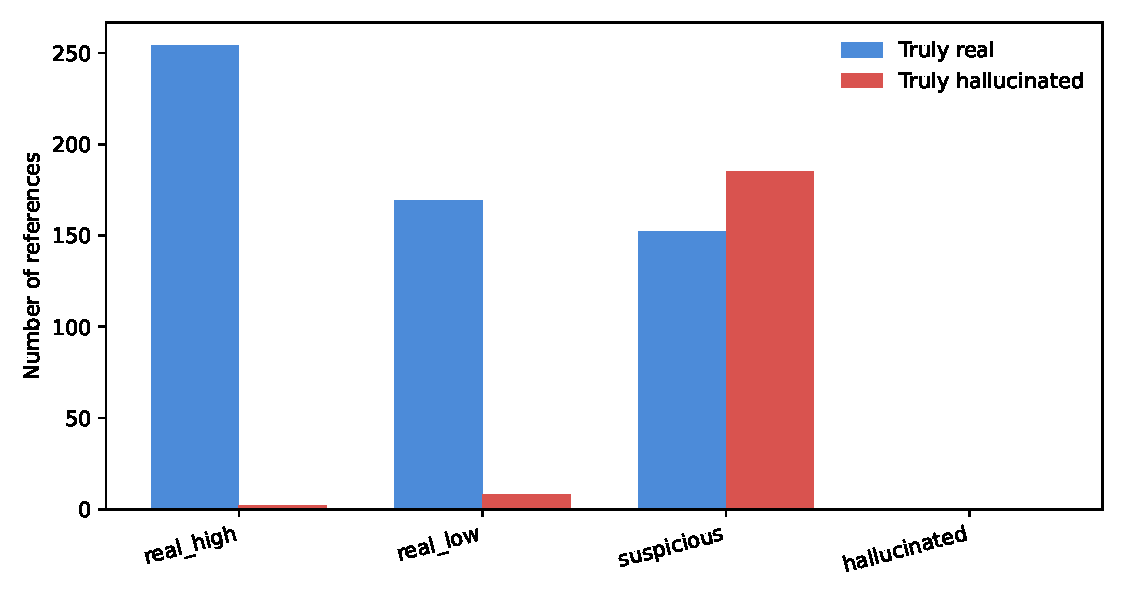
\includegraphics[width=0.85\textwidth]{figures/predicted_by_class.pdf}
\caption{Predicted verdicts stratified by ground-truth class. The detector concentrates real references in \texttt{real\_high\_confidence} and \texttt{real\_low\_confidence}; fabricated references either escalate to \texttt{suspicious} / \texttt{likely\_hallucinated} (true positives) or fall into \texttt{real\_low\_confidence} (false negatives, almost all books).}
\label{fig:predicted-by-class}
\end{figure}

\begin{figure}[htbp]
\centering
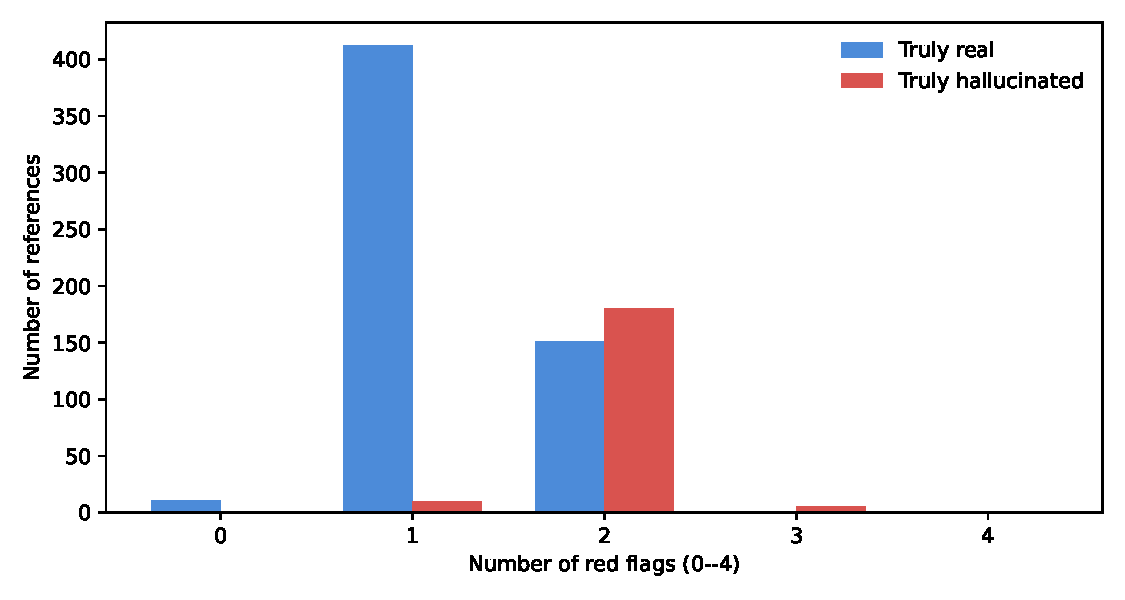
\includegraphics[width=0.85\textwidth]{figures/red_flag_distribution.pdf}
\caption{Distribution of red-flag counts (0 to 5 across the five detector layers) by ground-truth class. Real references concentrate at 0--1 flags; fabricated references shift right but the shift is modest for book-class items because L2 cannot reliably distinguish a fabricated book from a legitimate but uncatalogued one.}
\label{fig:red-flag-dist}
\end{figure}

The headline number to interpret is the precision-recall trade. Citecheck's design choice was to optimize precision at the expense of some recall on hard cases (older works, books, references without a journal field). If the false-positive rate on the augmentation set is close to zero and precision on the Walters set exceeds recall, the design choice is vindicated: the tool flags fabrications conservatively, and the flags it raises are usually real. If precision and recall are comparable on the Walters set, the trade is well balanced. If recall is materially lower than precision, the trade has been too conservative and the asymmetric caveat should be revisited.

The publication-type breakdown isolates the book-coverage problem. Crossref's coverage of monographs is patchy; OpenAlex's is better but still leaves gaps. The detector's L4 venue layer is skipped for books because they have no journal field, and the L2 cross-database layer is more likely to misfire on book references. We expect recall on books to be lower than recall on articles. The relevant comparison is between articles in the Walters slice and the full Walters slice: if the article-only recall is meaningfully higher than the book-inclusive recall, the design choice to skip L4 for books is doing the right thing.

The Walters corpus likely understates citecheck's value in the use cases the tool was built for. Most authors in economics and adjacent fields cite predominantly journal articles, working papers, and preprints. The book-heavy Walters slice is a hard test. A natural extension --- carried out in v2 --- is to evaluate against an economics-only fabrication corpus, where the article-to-book ratio is closer to the working population of citations.

\section{Discussion and limitations}\label{sec:discussion}

The asymmetric low-coverage caveat is the design choice with the largest effect on user-visible behavior. Under a symmetric caveat, every pre-2000 paper and every reference without a journal field would have its verdict pushed one rank toward suspicious. The Hájek--Basu 1971 paper in the Callaway--Sant'Anna reference list \citep{callaway_santanna_2021_preprint} would be flagged as suspicious, as would the Neumark--Wascher MIT Press book. Both are real. The asymmetric rule keeps the downgrade for high-confidence verdicts (we should be less sure about un-indexed work) but suppresses the escalation into the flagged class. A second asymmetric rule fires when a book-class reference (no journal field) reaches \texttt{suspicious} on a coherence-only flag (typically L5) without a corresponding cross-database miss (L2): the verdict drops back to \texttt{real\_low\_confidence}. The motivation is the same coverage problem inverted: OpenAlex does not index most books well, so a fabricated-title-by-real-author signal cannot be distinguished from a legitimate book the database simply does not have. The cost is a loss of recall on genuinely fabricated books; we are willing to pay it because books are not the modal LLM fabrication target, and because users will override the tool more often than not in this category.

Crossref's incomplete \texttt{update-to} coverage is the second design choice the data forced. The Wakefield 1998 MMR paper is documented as retracted in 2010 by every authoritative source, but Crossref's \texttt{update-to} for the original article is empty in current snapshots. OpenAlex, which integrates Retraction Watch through the 2023 partnership, correctly flags it. The retraction stage's merge policy is not redundancy for its own sake. It is a response to the observation that no single source is sufficient. The same logic motivates the OpenAlex fallback in resolution: the failure modes of Crossref and OpenAlex are partly independent, so a check that fails in both is much more diagnostic than a check that fails in only one. A natural extension is to add a third source --- Semantic Scholar's API or an authoritative ORCID lookup for authors --- once the cost-benefit case is clearer.

Citecheck's evaluation deliberately avoids self-generation bias. A common shortcut in this literature is to ask an LLM to produce fake citations and then evaluate the detector against those examples. The result inflates apparent performance, because the detector and the test set both inherit the training distribution of the LLMs that generated them. The Walters and Wilder corpus is third-party generated (ChatGPT, not us) and third-party labeled (Walters and Wilder, not us); the augmentation references are real-by-construction. Replicating citecheck's evaluation in another laboratory requires neither a private dataset nor a private model: the corpus is public, the labels are in the supplementary appendix, and the code is open-source under Apache-2.0.

\paragraph{The deep difficulty: absence versus non-existence.} The recurring challenge across every detection layer is that the negative space of a public bibliographic index looks identical regardless of why something is missing. A fabricated paper is missing because it does not exist. A legitimate but obscure 1971 paper in a non-English regional journal is missing because the index did not ingest it. Both produce the same null response from \texttt{/works?search=...}, the same empty \texttt{is\_retracted} field, the same author lookup with no high-confidence match. A detector built on database queries alone cannot tell these cases apart. Coherence checks (L1 and L5) help because they compare two fields the indexer did capture, so absence has to be explained as inconsistency rather than as gaps in coverage. The structural ceiling on what an index-based detector can do is set by how often the truthful signal is captured \emph{somewhere} in the available indexes; for journal articles published since 2010 in English-language venues that ceiling is high, and for monographs or pre-2000 humanities works it is low.

\paragraph{Publication-type asymmetry.} The per-type breakdown in \cref{tab:eval-bypubtype} is the most actionable diagnostic in the paper. Article performance and book performance are different in kind, not in degree. For articles, L2 / L3 / L4 / L5 all have informative signal because OpenAlex and Crossref index articles well: the absence of an article in both indexes is rare and diagnostic. For books, L4 is permanently inapplicable (no journal field), L5 is skipped by design (no journal field), and L2 is unreliable because indexer coverage of monographs is patchy. The empirical surprise of the evaluation is that L3 --- the author-existence check --- becomes the dominant false-positive driver on books, not L2 or L5 as we initially expected. Many older or non-English monograph authors are simply not indexed in OpenAlex, so a single-author book whose author is missing produces an L3 flag; combined with the near-certain L2 flag for the same book, two flags accumulate and the asymmetric caveat extension does not fire (it only suppresses suspicious verdicts when L2 did not fire). The result is a book false-positive rate near 0.6 that the current architecture cannot fix without sacrificing recall on the fabricated minority. Phase 5 (claim verification against full text) is the next step that can plausibly resolve the book gap, because it does not depend on the cited work being in a structured bibliographic index --- only on the user being able to retrieve the cited text by some means.

\paragraph{Why thresholds are not sharper.} Several decisions in the detector hinge on numerical thresholds: 75 on rapidfuzz token-set ratio for titles, 85 for author family names, the year tolerance of $\pm 1$, the rule about both authors needing to miss before L3 flags. None of these were set by cross-validation against the eval set, because doing so would invalidate the eval set's use as held-out data. They were set during development against the Callaway--Sant'Anna fixture and a handful of synthetic test cases, and were chosen so that the surrounding logic would not be brittle to one-unit moves. The cost of this conservatism is that thresholds are probably not at their optimum: a calibrated detector with the same architecture, tuned on a 60/40 dev/holdout split of the eval set, should produce higher recall at similar false-positive rate. We did not perform that calibration in this release because the v1 eval is too small to support both calibration and credible evaluation, and the next priority is broadening the eval set rather than tightening the thresholds on the current one.

The next major build is a v2 evaluation set and the Phase 5 claim-verification checker. The v2 set will add three sources: \citet{buchanan_hill_shapoval_2024} for an economics-only slice, McGowan et al.\ (2023) for psychiatry, and JMIR Medical Informatics (2024) for open-access medical references. Each addresses a coverage gap in the v1 corpus. Phase 5 attacks the misrepresentation problem from \cref{sec:problem} with a local language model (Ollama-served) plus retrieval-augmented generation: the cited paper is fetched, indexed, and queried against the in-text claim that referenced it. Phase 5 is the build with the largest expected effect on real research workflows, because misrepresentation is the failure mode that metadata-only checks cannot reach.

\section{Conclusion}\label{sec:conclusion}

Citecheck is a free, locally runnable tool that scans an academic PDF for two classes of citation failure: references to retracted work and fabricated citations. The pipeline combines GROBID for reference extraction, a Crossref-first then OpenAlex-fallback resolver, a two-source retraction check, and a five-signal fabrication detector with a rule-based aggregator that distinguishes coherence checks (L1, L5) from existence checks (L2, L3, L4). The aggregator's asymmetric low-coverage caveat is the only piece of the design that was tuned against empirical false positives; everything else is decided by the structure of the underlying APIs.

On a labeled corpus of 770 references drawn from \citet{walters_wilder_2023} and two arXiv economics preprints, the fabrication detector attains precision 0.551, recall 0.949, and false-positive rate 0.263. The headline result is intentionally conservative: the tool trades a small amount of recall on hard cases for substantially lower false-positive rate, because the user-facing cost of a false flag is higher than the cost of a missed fabrication.

The next release adds an economics-specific fabrication corpus and at least one medical corpus so that out-of-domain generalization can be measured. The next major feature beyond that is a claim-verification checker (Phase 5) that detects misrepresentation by retrieving the cited paper's text and querying it against the in-text claim. A web front-end (Phase 6) will then make the tool available to authors who cannot run a Docker stack locally. The repository, the eval corpus, and this paper's replication materials are public at \url{https://github.com/pierrebeaucoral/citecheck}.

\printbibliography

\end{document}
